
\begin{doubledpage}{theorem}{Inclusion-Exclusion}{
	Let $X$ be a set with a decomposition into smaller subsets, $X=\bigcup_{i\in I} U_i$. Let $U_J=\cap_{j\in J} U_i$. There exists an exact chain complex $CR^\bullet(\mathcal U)$ with $CR^\bullet(\mathcal U)=\bigoplus_{J\subset I, |J|=k} \mathcal F(U_J)$. }
	
\[
	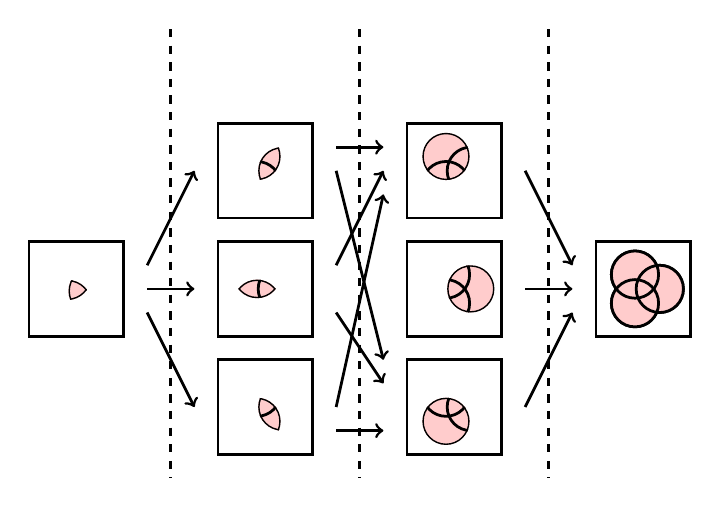
\begin{tikzpicture}[scale=.3]

\begin{scope}[shift={(-24,2)}]
\draw[line width = 1pt]  (13,-3) rectangle (17,-7);
\clip (-17:15.2947) circle[radius=1];
\clip (-18:16.477) circle[radius=1];
\clip (-21:15.6861) circle[radius=1];
\fill[red!20] (-17:15.2947) circle[radius=1];
\fill[red!20] (-18:16.477) circle[radius=1];
\fill[red!20] (-21:15.6861) circle[radius=1];
\draw[line width = 1pt] (-17:15.2947) circle[radius=1];
\draw[line width = 1pt] (-18:16.477) circle[radius=1];
\draw[line width = 1pt] (-21:15.6861) circle[radius=1];
\end{scope}\begin{scope}[shift={(15,-3)}]
\draw[line width = 1pt]  (-2,2) rectangle (2,-2);
\draw[line width = 1pt] (120:0.7) circle[radius=1];
\draw[line width = 1pt] (0:0.7) circle[radius=1];
\draw[line width = 1pt] (240:0.7) circle[radius=1];
\fill[red!20] (120:0.7) circle[radius=1];
\fill[red!20] (0:0.7) circle[radius=1];
\fill[red!20] (240:0.7) circle[radius=1];
\draw[line width = 1pt] (120:0.7) circle[radius=1];
\draw[line width = 1pt] (0:0.7) circle[radius=1];
\draw[line width = 1pt] (240:0.7) circle[radius=1];
\end{scope}\begin{scope}[shift={(7,2)}]
\draw[line width = 1pt]  (-2,2) rectangle (2,-2);
\clip (120:0.7) circle[radius=1];
\draw[line width = 1pt] (0:0.7) circle[radius=1];
\draw[line width = 1pt] (240:0.7) circle[radius=1];
\fill[red!20] (120:0.7) circle[radius=1];
\fill[red!20] (0:0.7) circle[radius=1];
\fill[red!20] (240:0.7) circle[radius=1];
\draw[line width = 1pt] (120:0.7) circle[radius=1];
\draw[line width = 1pt] (0:0.7) circle[radius=1];
\draw[line width = 1pt] (240:0.7) circle[radius=1];
\end{scope}\begin{scope}[shift={(7,-3)}]
\draw[line width = 1pt]  (-2,2) rectangle (2,-2);
\clip (0:0.7) circle[radius=1];
\draw[line width = 1pt] (120:0.7) circle[radius=1];
\draw[line width = 1pt] (240:0.7) circle[radius=1];
\fill[red!20] (120:0.7) circle[radius=1];
\fill[red!20] (0:0.7) circle[radius=1];
\fill[red!20] (240:0.7) circle[radius=1];
\draw[line width = 1pt] (120:0.7) circle[radius=1];
\draw[line width = 1pt] (0:0.7) circle[radius=1];
\draw[line width = 1pt] (240:0.7) circle[radius=1];
\end{scope}\begin{scope}[shift={(7,-8)}]
\draw[line width = 1pt]  (-2,2) rectangle (2,-2);
\clip (240:0.7) circle[radius=1];
\draw[line width = 1pt] (120:0.7) circle[radius=1];
\draw[line width = 1pt] (0:0.7) circle[radius=1];
\fill[red!20] (120:0.7) circle[radius=1];
\fill[red!20] (0:0.7) circle[radius=1];
\fill[red!20] (240:0.7) circle[radius=1];
\draw[line width = 1pt] (120:0.7) circle[radius=1];
\draw[line width = 1pt] (0:0.7) circle[radius=1];
\draw[line width = 1pt] (240:0.7) circle[radius=1];
\end{scope}\begin{scope}[shift={(-1,2)}]
\draw[line width = 1pt]  (-2,2) rectangle (2,-2);
\clip (120:0.7) circle[radius=1];
\clip (0:0.7) circle[radius=1];
\draw[line width = 1pt] (240:0.7) circle[radius=1];
\fill[red!20] (120:0.7) circle[radius=1];
\fill[red!20] (0:0.7) circle[radius=1];
\fill[red!20] (240:0.7) circle[radius=1];
\draw[line width = 1pt] (120:0.7) circle[radius=1];
\draw[line width = 1pt] (0:0.7) circle[radius=1];
\draw[line width = 1pt] (240:0.7) circle[radius=1];
\end{scope}\begin{scope}[shift={(-1,-3)}]
\draw[line width = 1pt]  (-2,2) rectangle (2,-2);
\clip (120:0.7) circle[radius=1];
\clip (240:0.7) circle[radius=1];
\draw[line width = 1pt] (0:0.7) circle[radius=1];
\fill[red!20] (120:0.7) circle[radius=1];
\fill[red!20] (0:0.7) circle[radius=1];
\fill[red!20] (240:0.7) circle[radius=1];
\draw[line width = 1pt] (120:0.7) circle[radius=1];
\draw[line width = 1pt] (0:0.7) circle[radius=1];
\draw[line width = 1pt] (240:0.7) circle[radius=1];
\end{scope}\begin{scope}[shift={(-1,-8)}]
\draw[line width = 1pt]  (-2,2) rectangle (2,-2);
\clip (0:0.7) circle[radius=1];
\clip (240:0.7) circle[radius=1];
\draw[line width = 1pt] (120:0.7) circle[radius=1];
\fill[red!20] (120:0.7) circle[radius=1];
\fill[red!20] (0:0.7) circle[radius=1];
\fill[red!20] (240:0.7) circle[radius=1];
\draw[line width = 1pt] (120:0.7) circle[radius=1];
\draw[line width = 1pt] (0:0.7) circle[radius=1];
\draw[line width = 1pt] (240:0.7) circle[radius=1];
\end{scope}




\draw[line width = 1pt][dashed] (-5,8) -- (-5,-11);
\draw[line width = 1pt][dashed] (3,8) -- (3,-11);
\draw[line width = 1pt][dashed] (11,8) -- (11,-11);
\draw[line width = 1pt,->] (-6,-2) -- (-4,2);
\draw[line width = 1pt,->] (-6,-3) -- (-4,-3);\draw[line width = 1pt,->] (-6,-4) -- (-4,-8) ;\draw[line width = 1pt,->](2,3) -- (4,3);\draw[line width = 1pt,->] (2,2) -- (4,-6) ;\draw[line width = 1pt,->](2,-9) -- (4,-9) ;\draw[line width = 1pt,->](2,-8) -- (4,1);\draw[line width = 1pt,->] (2,-4) -- (4,-7) ;\draw[line width = 1pt,->](2,-2) -- (4,2) ;\draw[line width = 1pt,->](10,-8) -- (12,-4);\draw[line width = 1pt,->] (10,-3) -- (12,-3) ;\draw[line width = 1pt,->](10,2) -- (12,-2);
\end{tikzpicture}
\]
We will prove this theorem by using the tools of homological algebra, and induct on the size of $I$. 
\begin{definition}
	Let $\mathcal U=\{U_i\}_{i\in I}$ be a collection of subsets which cover $X$. Denote by 
	$\mathcal U_{\cap}:= \{U_j\}_{}$
\end{definition}

A covering $\mathcal U=\{U_i\}$ of $X$  is a collection of subsets $U_i\subset X$ so that  \[X=\bigcup_{i\in I} U_i.\]
To each covering of $X$ we will create an \emph{resolution complex} $CR_\bullet(\mathcal U)$.
\begin{definition}
Let $\mathcal U=\{U_i\}_{i\in I}$ be a covering of $X$. For each $J\subset I$, define the subset $U_J:=X\cap (\bigcap_{i\in J} U_i)$.
Suppose that $J$ and $K$ differ by a single index. We will then write $J\lessdot K$. Notice that whenever $K\gtrdot J$ we have an inclusion map $i_{K\gtrdot J}:U_K\to U_J$, and therefore we get an associated map 
\[i_{K\gtrdot J}^*: \mathcal F (U_J)\to \mathcal F(U_K).\]
We define the chain groups 
\[CR^k(\mathcal U):=\bigoplus_{K\subset I, |K|=k} \mathcal F(U_K)\]
and define the differential map to be
\[d^k_{CR}:=\bigoplus_{K\gtrdot J} i_{K\gtrdot J}^*.\]
\end{definition}
We will show that this gives us a chain complex by constructing it in a different fashion. 

\begin{lemma}
	Let $\hat U_1$ be the elements of $X$ which only belong to $U_1$,   Let $\mathcal U_X=\{U_i\}_{i\in I}$ be a cover of $X$. Let $\mathcal U_{\cap}=\{U_i\cap U_1\}_{1\neq i\in I} $ be a cover for $U_1\setminus \hat A_1$. Let $\mathcal U_{\setminus}=\{U_i\}_{1\neq i\in I}$ be a cover for $X \setminus \hat U_1$.
	 Then there is a natural maps $i_{J}: \bigcap_{i\in J}(U_i\cap U_1 )\to \bigcap_{i\in J}(U)i)$ for each $J$, inducing a map 
	\[i^*: CR_\bullet(\mathcal U_\setminus)\to CR_\bullet(\mathcal U_\cap)\]
	and $CR_\bullet(\mathcal U_X)=\cone(i^*)\oplus (\mathcal F(\hat U_1)\to \mathcal F(\hat U_1)$
\end{lemma}

As always, a diagram explains the core concept of this proof:
\[\begin{tikzpicture}[commutative diagrams/every diagram]
\fill[red!10] (0,3) -- (-2.5,-0.5) -- (1.5,-0.5) -- (4,3) -- cycle;
\fill[blue!10] (-1.5,5.5) -- (-4,2) -- (0,2) -- (2.5,5.5) -- cycle;
\matrix[matrix of math nodes, name=m, commutative diagrams/every cell, row sep= 20, column sep = 30] {
\; & A_{12} & A_1 \\
			&\oplus&\oplus\\
A_{123}& A_{13}& A_2 & X\\
			&\oplus&\oplus\\
& A_{23} & A_3 \\};
\path[commutative diagrams/.cd, every arrow, every label]
(m-3-1) edge(m-1-2) edge (m-3-2) edge (m-5-2)
(m-1-2) edge(m-1-3) edge (m-3-3) 
(m-3-2) edge(m-1-3) edge (m-5-3) 
(m-5-2) edge(m-3-3) edge (m-5-3) 
(m-5-3) edge(m-3-4) 
(m-3-3) edge(m-3-4) 
(m-1-3) edge(m-3-4) 
;
\node at (1.5,7) {$CR_\bullet(\mathcal U_\cap \oplus A_1)$};
\node at (5,4) {$CR_\bullet(\mathcal U_\cup\oplus A_1)$};
\draw[->] (3,7) -- (4.5,4.5);
\end{tikzpicture}\]

\begin{corollary}
The homology of the resolution complexes are trivial: $H_\bullet(CR_\bullet(\mathcal U))=0$, i.e. $CR_\bullet(\mathcal U)$ is exact. 
\end{corollary}
\begin{proof}
We again prove by induction on the size of the cover. As a base case, we can let  $\mathcal U=\{X\}$, then $H_\bullet(\mathcal U)=0$ trivially. \\
Now assume that we know by induction that $CR_\bullet(\mathcal U_\cap)$ and $ CR_\bullet(\mathcal U_\cup)$ have trivial homology. Since the cone of exact chain complexes is exact, we get $CR_\bullet(\mathcal U)$ is exact. 
\end{proof}
\end{doubledpage}